\documentclass[11pt]{article}
\usepackage[margin=1in]{geometry}
\usepackage{booktabs}
\usepackage{amsmath,amssymb}
\usepackage{graphicx}
\usepackage{hyperref}

% Paper-facing assets are copied through tools/export_manuscript_assets.py,
% which records their source paths and hashes.
\graphicspath{
  {../generated/figures/adaptive_h/}
}

\title{Oracle Adaptive Bandwidth Diagnostics for CKME-Based Conformal Prediction}
\author{}
\date{\today}

\begin{document}
\maketitle

\paragraph{Status.}
This report records the fixed-versus-oracle adaptive-bandwidth diagnostics.
The numerical results predate the locked estimator and calibration protocol in
\texttt{PROTOCOL.md}; they are retained as mechanism evidence rather than as
final manuscript results. The implementable plug-in method is defined separately
in \texttt{experiments/adaptive\_h/planned\_final\_benchmark\_spec.md} as
per-site sample standard deviation followed
by Nadaraya--Watson smoothing. Its final results should be reported only after a
protocol-aligned run.

\section{Question}

The standard CKME conditional CDF estimator uses a single CV-tuned smooth-indicator
bandwidth. Under heterogeneous conditional response scales, the effective
bandwidth is \(h/s(x)\), so a fixed \(h\) can oversmooth low-scale regions and
undersmooth high-scale regions. The oracle diagnostic asks whether replacing the
scalar bandwidth with
\[
  h(x)=c\,s(x)
\]
improves interval efficiency and bin-wise coverage stability without changing
the conformal calibration layer.

\section{Diagnostic setup}

The existing outputs compare a fixed scalar bandwidth with an oracle adaptive
bandwidth on four one-dimensional data-generating processes:
\texttt{wsc\_gauss}, \texttt{gibbs\_s1}, \texttt{exp1}, and
\texttt{nongauss\_A1L}. The reported quantities are marginal coverage, bin-wise
coverage deviation, mean interval width, and Winkler interval score. Common
random numbers across arms support paired comparisons.

Because these outputs were produced before the current protocol lock, their role
is limited to checking the scale-normalization mechanism. They should not be used
as final evidence for the paper's finite-sample coverage claim.

\section{Fixed-bandwidth baseline}

\begin{table}[h!]
\centering
\caption{Fixed-bandwidth diagnostic summary. Target marginal coverage is
\(1-\alpha=0.90\).}
\label{tab:exp1}
\resizebox{\linewidth}{!}{%
% Exp1 fixed-h baseline. Target marginal coverage = 0.90.
% Cell format: median (sd across macroreps) for binwise stats; mean (sd) for width and interval score.
\begin{tabular}{lrrrrrrr}
\toprule
DGP & $K$ & marginal cov & worst-bin $|c-(1-\alpha)|$ & mean-bin $|c-(1-\alpha)|$ & cov range & mean width & mean IS \\
\midrule
wsc\_gauss & 50 & 0.900 (0.010) & 0.148 (0.046) & 0.060 (0.009) & 0.248 (0.047) & 2.126 (0.083) & 2.935 (0.138) \\
gibbs\_s1 & 50 & 0.903 (0.011) & 0.106 (0.037) & 0.044 (0.007) & 0.193 (0.047) & 2.200 (0.065) & 2.818 (0.104) \\
exp1 & 50 & 0.898 (0.010) & 0.159 (0.039) & 0.065 (0.008) & 0.259 (0.041) & 2.099 (0.134) & 3.231 (0.259) \\
nongauss\_A1L & 50 & 0.903 (0.013) & 0.136 (0.041) & 0.056 (0.009) & 0.236 (0.045) & 3.179 (0.275) & 5.549 (0.774) \\
\bottomrule
\end{tabular}

}
\end{table}

\section{Oracle adaptive bandwidth}

The oracle arm sets \(h(x)=c\,s(x)\), with a small numerical floor where the
scale approaches zero. This arm isolates the mechanism of response-scale
normalization without introducing scale-estimation error.

\subsection{Paired comparison with fixed bandwidth}

\begin{table}[h!]
\centering
\caption{Oracle minus fixed paired comparison. Negative interval-score
differences favor the oracle arm.}
\label{tab:exp2}
\resizebox{\linewidth}{!}{%
% Exp2 paired comparison. Target marginal coverage = 0.90.
% Worst-bin / marginal cov: median across macroreps. Width: mean across macroreps. Delta = oracle - fixed (negative is better).
\begin{tabular}{l ccc ccc cc}
\toprule
 & \multicolumn{3}{c}{Worst-bin $|c-(1-\alpha)|$} & \multicolumn{3}{c}{Mean width} & \multicolumn{2}{c}{Marginal cov} \\
\cmidrule(lr){2-4} \cmidrule(lr){5-7} \cmidrule(lr){8-9}
DGP & fixed & oracle & $\Delta$ & fixed & oracle & ratio & fixed & oracle \\
\midrule
wsc\_gauss & 0.148 & 0.100 & -0.048 & 2.126 & 2.114 & 0.99 & 0.900 & 0.902 \\
gibbs\_s1 & 0.106 & 0.098 & -0.008 & 2.200 & 2.189 & 1.00 & 0.903 & 0.901 \\
exp1 & 0.159 & 0.091 & -0.068 & 2.099 & 2.400 & 1.14 & 0.898 & 0.898 \\
nongauss\_A1L & 0.136 & 0.105 & -0.032 & 3.179 & 2.988 & 0.94 & 0.903 & 0.901 \\
\bottomrule
\end{tabular}

}
\end{table}

\begin{figure}[h!]
\centering
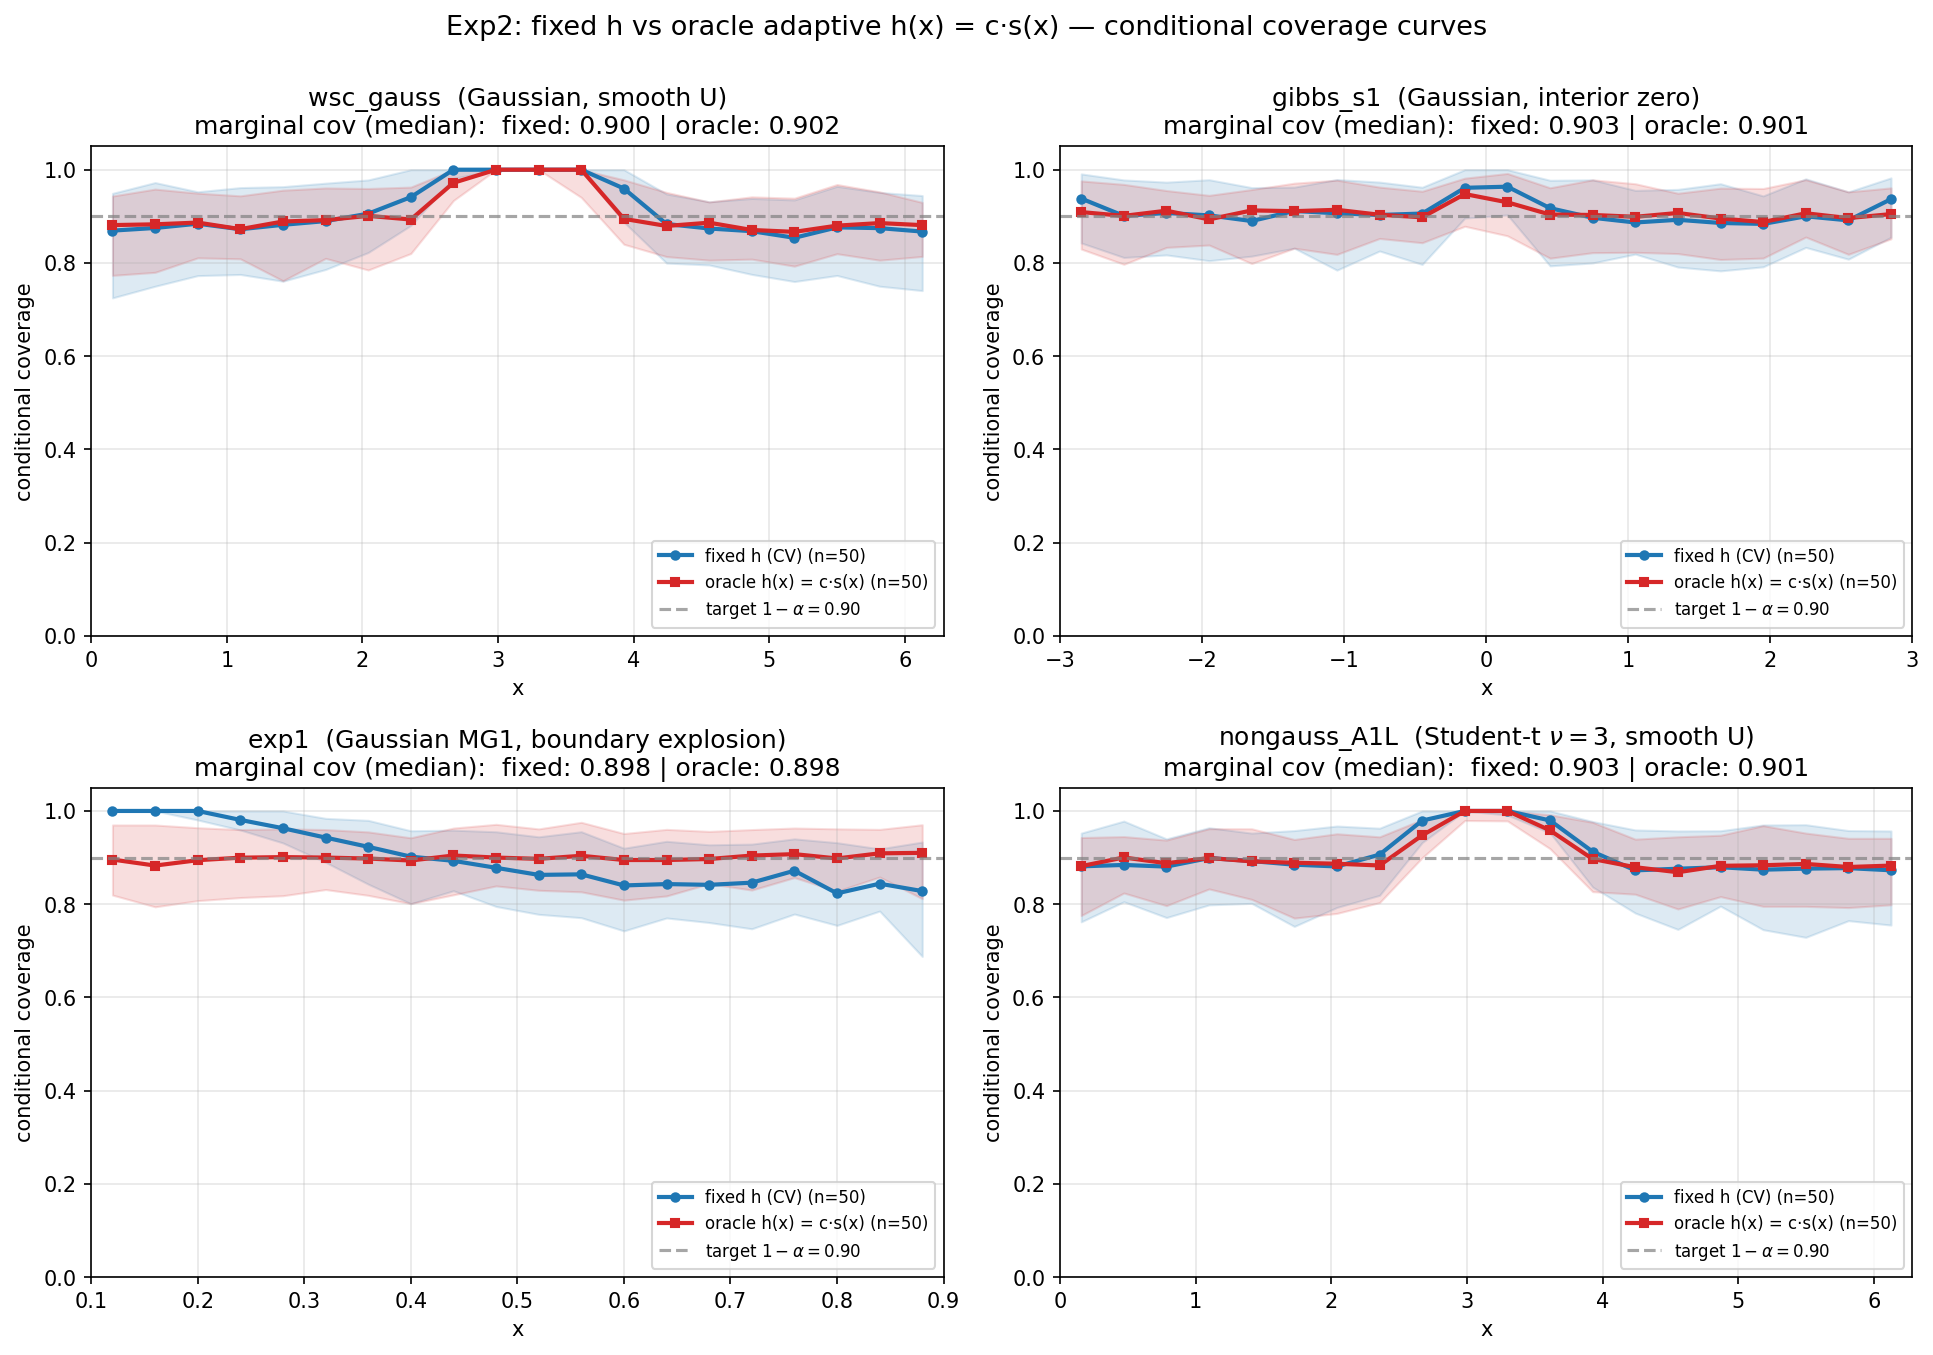
\includegraphics[width=0.85\linewidth]{exp2_oracle_vs_fixed_coverage.png}
\caption{Bin-wise coverage curves for the oracle and fixed-bandwidth arms.}
\label{fig:exp2}
\end{figure}

\subsection{Sensitivity to the multiplier \(c\)}

\begin{table}[h!]
\centering
\caption{Oracle multiplier sweep on \texttt{nongauss\_A1L}.}
\label{tab:exp3}
\resizebox{\linewidth}{!}{%
% Exp3 c-sweep on nongauss_A1L. Target marginal coverage = 0.90.
% Cell format: median (sd) for binwise stats; mean (sd) for width and IS.
\begin{tabular}{lrrrrrr}
\toprule
arm & $c$ & marginal cov & worst-bin $|c-(1-\alpha)|$ & mean-bin $|c-(1-\alpha)|$ & mean width & mean IS \\
\midrule
fixed & --- & 0.903 (0.013) & 0.136 (0.041) & 0.056 (0.009) & 3.179 (0.275) & 5.549 (0.774) \\
c0.3 & 0.3 & 0.899 (0.013) & 0.115 (0.034) & 0.052 (0.008) & 3.129 (0.226) & 5.410 (0.758) \\
c0.5 & 0.5 & 0.901 (0.012) & 0.113 (0.028) & 0.050 (0.007) & 3.037 (0.178) & 5.341 (0.752) \\
c1 & 1 & 0.901 (0.012) & 0.105 (0.021) & 0.046 (0.007) & 2.988 (0.150) & 5.276 (0.744) \\
c2 & 2 & 0.900 (0.012) & 0.104 (0.020) & 0.042 (0.007) & 3.009 (0.153) & 5.251 (0.742) \\
\bottomrule
\end{tabular}

}
\end{table}

\begin{figure}[h!]
\centering
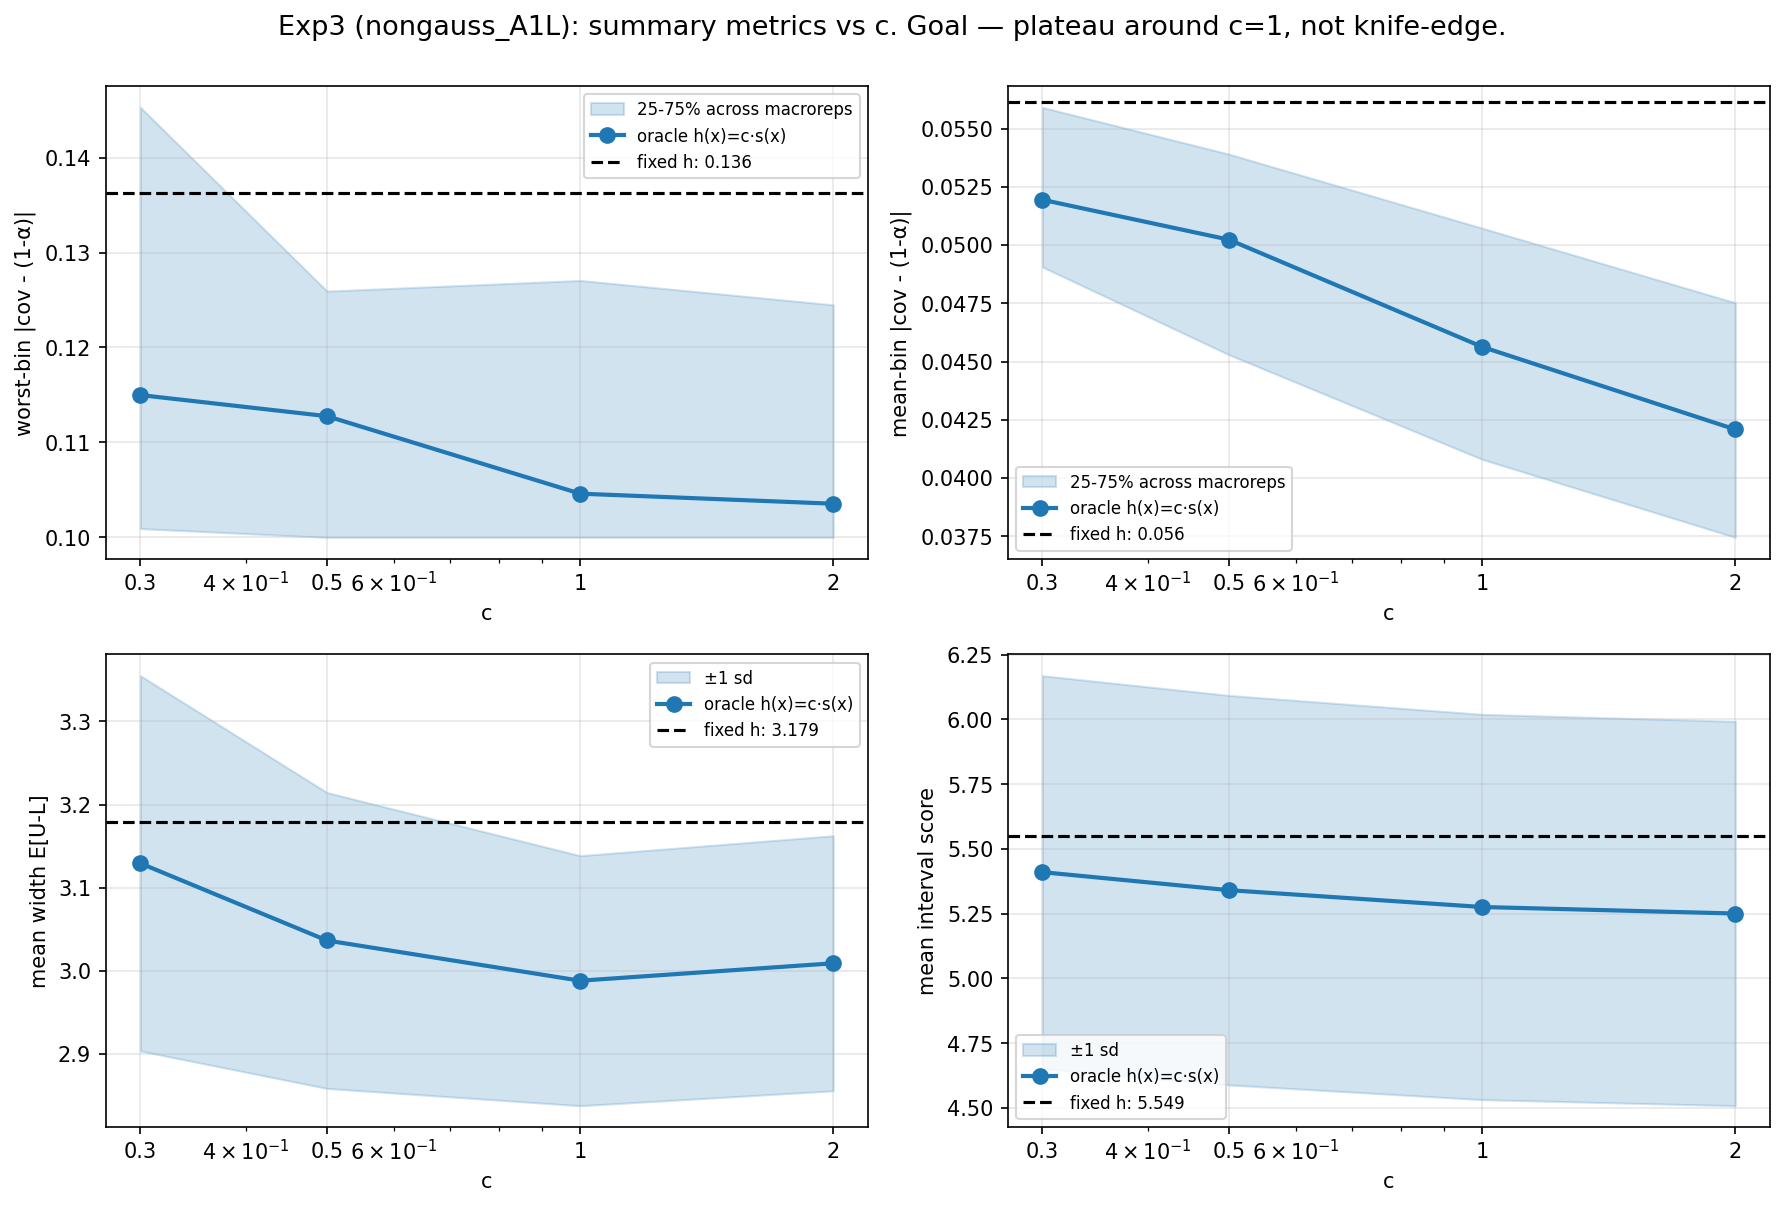
\includegraphics[width=0.70\linewidth]{exp3_oracle_c_sweep_metrics.png}
\caption{Worst-bin deviation, mean width, and interval score across oracle
multiplier values.}
\label{fig:exp3}
\end{figure}

\section{Interpretation}

The existing outputs provide diagnostic support for the oracle mechanism:
normalizing the smooth-indicator bandwidth by the local response scale improves
bin-wise stability and paired interval score relative to a fixed bandwidth in
the tested settings. The appropriate manuscript claim remains narrower than the
raw numerical pattern: these results motivate the adaptive rule and identify
useful diagnostics, but final numerical claims require rerunning the fixed,
oracle, and sample-SD plug-in arms under the locked protocol.

\section{Next evidence step}

The next paper-facing experiment should use the single implementable plug-in
defined in
\path{experiments/adaptive_h/final_benchmark_spec.md}: compute the
sample standard
deviation at each replicated Stage~1 site, smooth those sitewise estimates by
Nadaraya--Watson regression, and use \(h(x)=c\widehat s(x)\). The run should use
the calibration and reporting rules in \texttt{PROTOCOL.md}, save raw scores and
scale diagnostics, and produce a manifest connecting every table and figure to
its source outputs.

\end{document}
